\section*{Problem 8}
	\begin{proof}
		Denote that $X(G) = 1$ means the crossing number of $G$ is 1.\\
		We can find one example for $X(K_{3,3}) \leq 1$.
		\begin{center}
			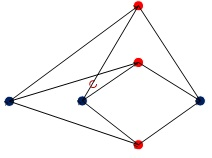
\includegraphics[width=0.4\textwidth]{K33.jpg}
		\end{center}
		If we show that $X(K_{3,3}) \neq 0$ i.e. $K_{3,3}$ is not planar, then $X(K_{3,3}) = 1$. We can prove this by applying \textit{Euler formula} as the \hyperref[problem 6]{Problem 6}. Therefore, $X(K_{3,3}) = 1$.\\
		Similarly, we can find $X(K_{3,4}) \leq 2$(note that $X(K_{4,3}) = X(K_{3,4})$).
		\begin{center}
			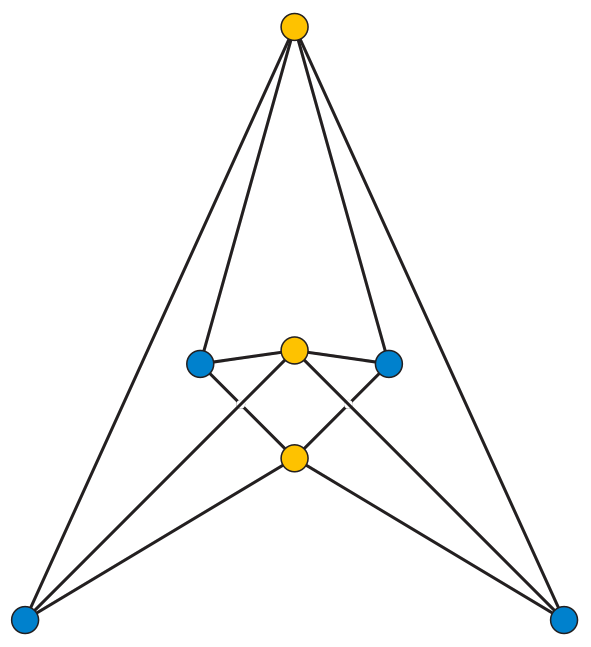
\includegraphics[width=0.4\textwidth]{K43.png}
		\end{center}
		Suppose $X(K_{3,4}) = 1$. Remove one blue vertex(in 4-node set) who occurs the crossing(note that crossing occurs between 4 vertices). Then there is no crossing, the graph forms $K_{3,3}$. i.e. $X(K_{3,3}) = 0$, contradiction. Therefore, $X(K_{3,4}) > 1$, so $X(K_{3,4}) = 2$.\\
		Similarly, we can find $X(K_{4,4}) \leq 4$.
		\begin{center}
			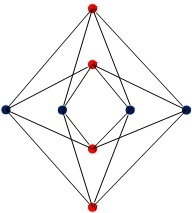
\includegraphics[width=0.4\textwidth]{K44.jpg}
		\end{center}
		Suppose $X(K_{4,4}) = 3$. Note taht crossing needs at least 4 vertices. Since $K_{4,4}$ has 8 vertices, there is at least one vertex which occurs at least 2 crossing. It is impossible to create 3 crossings with only 8 nodes so that every node participates in the crossing only once. So choose the node who occurs 2 crossing and remove it. Then the graph is $K_{3,4}$ with 1 crossing, contradiction. Therefore, $X(K_{4,4}) > 3$, so $X(K_{4,4}) = 4$.\\
	\end{proof}